\documentclass[a4paper]{article}
\usepackage{array}  
\usepackage{graphicx}
\graphicspath{ {./images/} }
\usepackage[table]{xcolor}% http://ctan.org/pkg/xcolor
\usepackage{geometry}
\geometry{margin=1.25in}
\usepackage{hhline}
\usepackage{environ}
\usepackage{longtable}
 %\geometry{
 %a4paper,z
 %total={170mm,257mm},
 %left=40mm,
 %right=40mm
 %}
 \newcommand{\colWidth}{141mm}

\begin{document} 
\section*{Demo day: \textit{(Demo 3)} Group \textit{(11 - FE.ED)}}

% ------------GOALS----------

\begin{center}
\begin{tabular}{|p{\colWidth}|}
	\hline
	\cellcolor{blue!25}\large
	\textbf{What were your goals?}
	\\ \hline
	\vtop to 180mm{
Our goals this time involved our sensors interacting with the environment. We categorised our goals into 3 main areas the robotics, server and  web app.
Our goals for each were as follows: 

 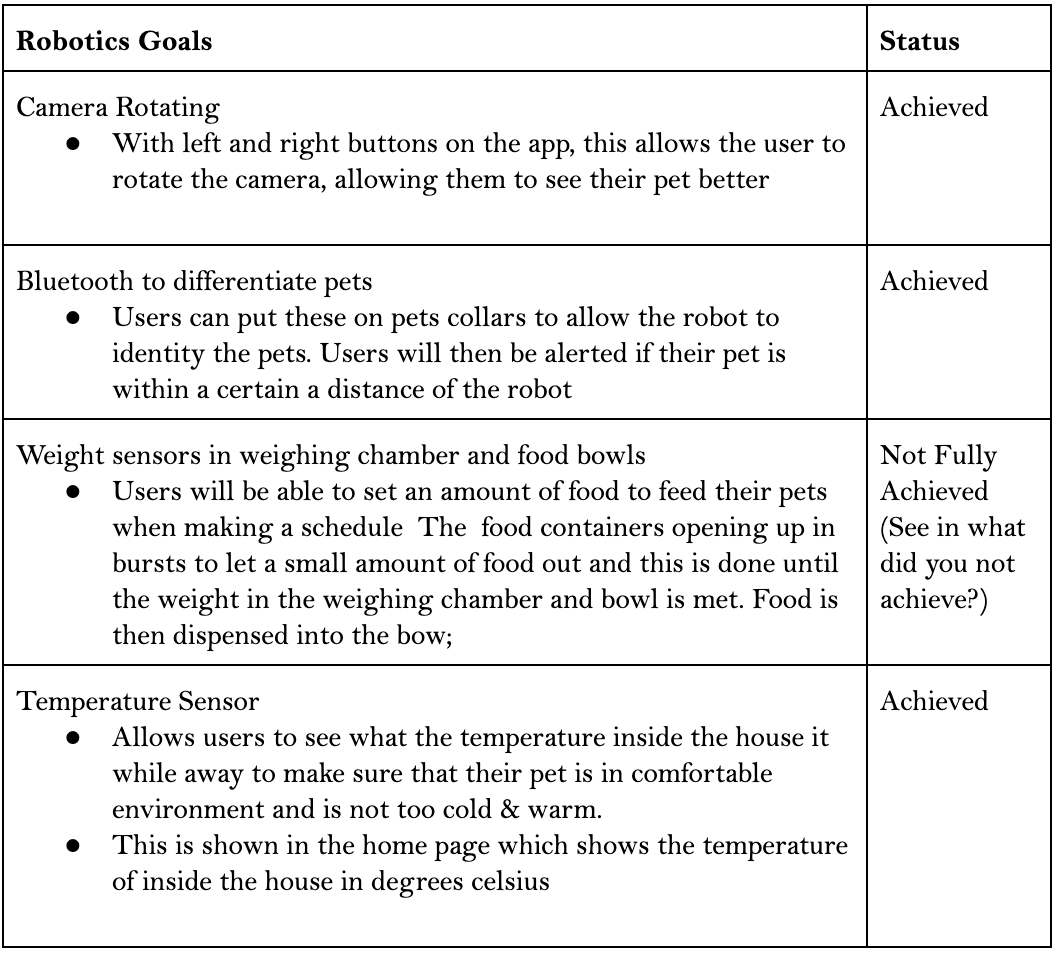
\includegraphics[width=10cm]{robot.png}
 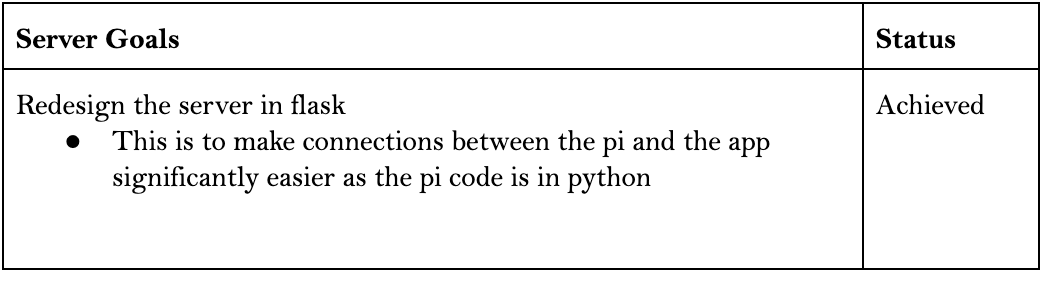
\includegraphics[width=10cm]{server.png}
 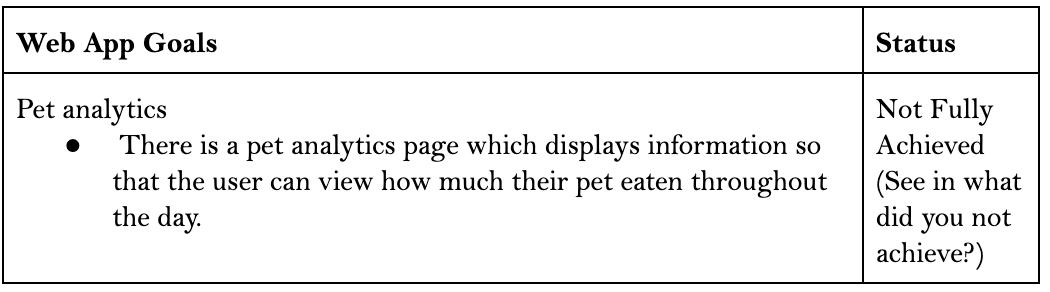
\includegraphics[width=10cm]{app.png}
  }
  \\
  \hline
\end{tabular}
\vskip 5mm


% ------------ORGANISATION----------

\begin{tabular}{|p{\colWidth}|}
	\hline
	\cellcolor{blue!25}\large
	\textbf{Summarise how your group organised the workload to achieve your goals.}
	\\ \hline
	\vtop to 30mm{
We used a sprint setup to try and maximize our efficiency at getting tasks done. We broke down our milestones into smaller independent tasks. This allowed us to isolate the specific tasks we needed to do. 
To try and make communication easier we tried to work together at the same time, whilst this occasionally was a little bit slower than doing it independently.  This meant that there was a some overlap in what we all worked on.


  }
  \\
  \hline
\end{tabular}
\vskip 5mm

% ------------ACHIEVEMENTS----------

\begin{tabular}{|p{\colWidth}|}
	\hline
	\cellcolor{blue!25}\large
	\textbf{What were your main achievements?}
	\\ \hline
	\vtop to 60mm{
Our main achievements were as follows:
\begin{itemize}
\item Setting up Bluetooth to differentiate pets, this then sends users an email alert if their pet is within a certain distance
\item Redesigning the server from Spring to Flask. This has allowed to simplify the server as Flask is a lot more light weight for our needs .
\item Temperature sensor which allows us to record the temperature of the room and display it in the app so the user knows whether their pet is in a comfortable environment.
\item Setting up a circuit connecting the arduino to the force sensitive resistor. We can then access this data through the raspberry pi.
\end{itemize}
  }
  \\
  \hline
\end{tabular}
\vskip 5mm

% ------------NOT ACHIEVED----------

\begin{tabular}{|p{\colWidth}|}
	\hline
	\cellcolor{blue!25}\large
	\textbf{What did you not achieve? Briefly explain why.}
	\\ \hline
	\vtop to 100mm{
\textbf{Note: Weight sensors in weighing chamber}
We were able to set up a circuit using a force sensitive resistor, connected to an arduino. Through connecting to the the raspberry pi, we are able to obtain a reading from the force sensitive resistor. Through tweaking the size of the resistor, the resistor can accurately detect differences when the pressure on it changes. \par
However, when testing the force sensitive resistor, we realised that it would not operate accurately in the current weighing chamber we had. After testing, we found that the pressure fluctuated wildly when at an angle. \par
To resolve this, we have decided to try and alter our design to allow us to have the force sensitive resistor flat. This means we will be able to gain more accurate readings. A further consideration is that when the weights are placed on the resistor, the force they apply is often not centralised and as a result the readings can often not be wholly accurate. From looking at similar designs, we identified a solution to this problem. Taking inspiration from a previous design, it is possible to force the pressure to a specific part of the resistor. We intend to use this for our bowl design for our next demo. 
\par
\par
\vspace{5mm}
\textbf{Note: Pet Analytics}
We were able to set up the front end for pet analytics with dummy data using a library called Canvas JS. We have graphs which will show how much their pet is eating versus  how much their pet is expected to eat. However as we could not get accurate readings from the force sensitive resistor, we could not send any data to the app. \par
\par
\vspace{5mm}
Unfortunately due to the research between weighing scales and pressure sensors we were unable to design and 3d print the bowls. This is because we were researching different weight scales and decided to go for the pressure sensor as it is more low profile and cost effective than the weighing scales.

  }
  \\
  \hline
\end{tabular}
\vskip 5mm

% ------------QUANTITIVE----------

\begin{tabular}{|p{\colWidth}|}
	\hline
	\cellcolor{blue!25}\large
	\textbf{Include any quantitative data you have collected (this can be a graph/table with a few words)}
	\\ \hline
	\vtop to 50mm{
	We've tested the force sensitive resistor on an incline. During testing we realised that the incline led to inaccurate readings. This is because the force of the food is not evenly distributed on the force sensitive resistor. We’ve also had the problem where there is a maximum amount of pressure the force sensitive resistor, the readings from the resistor become the same values. To try and solve this we've decided to develop and tests a flat weighing chamber. To solve the force of food being evenly distributed, we also have to find a way to force the food on the central part of the resistor.
	
	\vspace{5mm}
We decided to not do any quantitative analysis and user testing on the web app this demo as we have not added much to app and we would like to finalise the app before we do user testing.


  }
  \\
  \hline
\end{tabular}
\vskip 5mm
% ------------NEXT STEPS----------

\begin{tabular}{|p{\colWidth}|}
	\hline
	\cellcolor{blue!25}\large
	\textbf{Say briefly what changes you will make to your plan for the next demo.}
	\\ \hline
	\vtop to 45mm{
As we have not achieved all our milestones, we would like to redesign the weighing chamber to allow us to get accurate readings of the food and also send these readings to the pet analytics page.

\vspace{5mm}

For the next demo we will have the bowls 3D printed and designed as well as bowl flaps. We will also experiment with object recognition with the camera to see if we can get it rotating with the movement of the pet via Bluetooth. As we have had a problem with the doors of the food containers not closing properly, we would like to implement a switch to let the user know if a food container door has not shut fully so they can fix it.

}
  \\
  \hline
  
\end{tabular}

\end{center}
  
\end{document}